\documentclass[green, cn, normal]{elegantnote}

\graphicspath{{./figures/}}

\title{Geometry of Linear Algebra}
\author{\href{https://monkey-knight.github.io/}{monkey knight}}
\version{1.00}


\begin{document}
	\maketitle
	
	线性代数的基本问题就是解 $n$ 维方程组。例如:
	\[
	\begin{matrix}
	2x - y = 0 \\
	-x + 2y = 3
	\end{matrix}
	\]
	在线性代数的第一节课,我们将以三种方式来看待这个问题。
	
	上面的方程组是二维的($n=2$)。通过添加一个变量 $z$ 我们就能将其扩展为三维。
	
	\section{Row Picture}
	
	画出满足每个方程的所有的点。图的交点(前提是它们能够相交)就是方程组的解。从图 \ref{fig:intersection} 我们能够看出方程组的解是 $x=1$,$y=2$。
	
	\begin{figure}[!htbp]
		\centering
		\includegraphics[scale=0.6]{1.png}
		\caption{$2x-y=0$ 和 $-x + 2y = 0$ 在点($1, 2$)处相交}
		\label{fig:intersection}
	\end{figure}

	我们将这个解代入到原方程组中去检查:
	\[
	\begin{matrix}
	2 \cdot 1 - 2 = 0 \\
	-1 + 2 \cdot 2 = 3
	\end{matrix}
	\]
	
	三维方程组的解通常是三个平面的交点(前提是它们相交)。
	
	\section{Column Picture}
	
	通过将方程组中列的系数转换成向量,我们可以将方程组写成一个等式:
	\[
	x \begin{bmatrix}
	2 \\ -1
	\end{bmatrix} + y \begin{bmatrix}
	-1 \\ 2
	\end{bmatrix} = \begin{bmatrix}
	0 \\ 3
	\end{bmatrix}
	\]
	
	给定两个向量 $\textbf{c}$ 和 $\textbf{d}$ 以及标量 $x$ 和 $y$,那么 $x\textbf{c} + y \textbf{d}$ 就称为向量 $\textbf{c}$ 和 $\textbf{d}$ 的线性组合(\textbf{linear combination})。线性组合是这门课中非常重要的思想。
	
	从几何上看,我们是想要找到这样的数字 $x$ 和 $y$,使得 $x$ 个向量 $\begin{bmatrix}
	2 \\ -1
	\end{bmatrix}$ 的拷贝加上 $y$ 个向量 $\begin{bmatrix}
	-1 \\ 2
	\end{bmatrix}$ 的拷贝等于向量 $\begin{bmatrix}
	0 \\ 3
	\end{bmatrix}$。正如我们从图 \ref{fig:vector} 中看到的,$x=1$ 和 $y=2$,(这也与 Row Picture 中的结论相吻合)。
	
	\begin{figure}[!htbp]
		\centering
		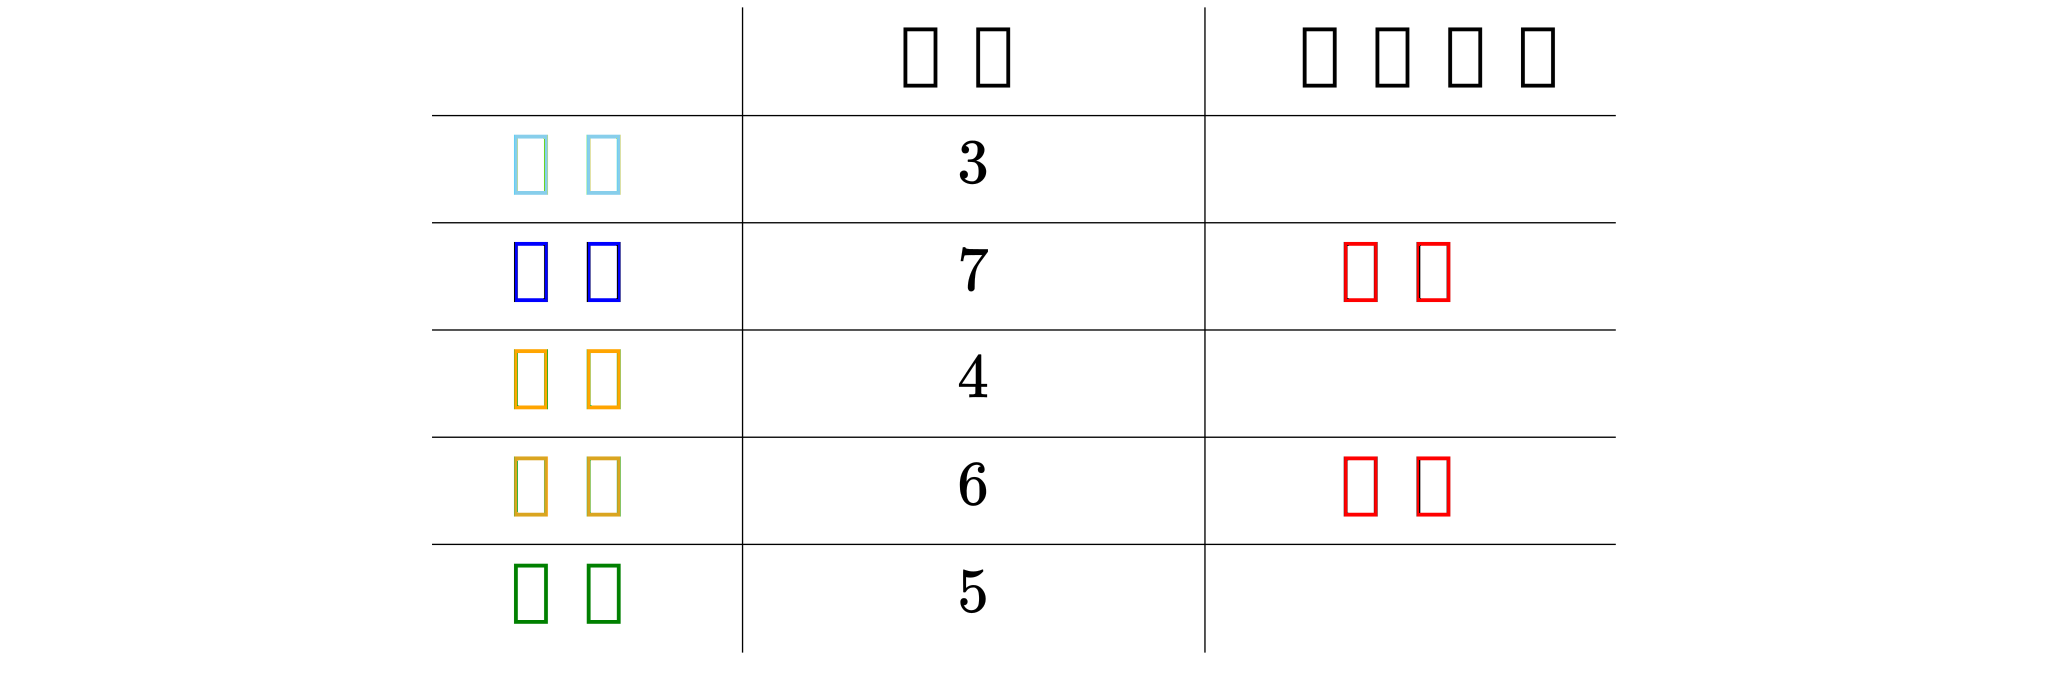
\includegraphics[scale=0.6]{2.png}
		\caption{列向量的 linear combination 等于向量 $\textbf{b}$}
		\label{fig:vector}
	\end{figure}

	在三维情况下,我们就需要找到三个三维向量的线性组合使得结果为 $\textbf{b}$。
	
	\section{Matrix Picture}
	
	我们通过矩阵和向量将上述的方程组写成一个等式:
	\[
	\begin{bmatrix}
	2 & -1 \\
	-1 & 2
	\end{bmatrix} \begin{bmatrix}
	x \\
	y
	\end{bmatrix} = \begin{bmatrix}
	0 \\ 3
	\end{bmatrix}
	\]
	
	矩阵 $A = \begin{bmatrix}
	2 & -1 \\
	-1 & 2
	\end{bmatrix}$ 叫做系数矩阵(\textbf{coefficient matrix}),向量 $\textbf{x} = \begin{bmatrix}
	x \\
	y
	\end{bmatrix}$ 是未知数,等式右边的值构成了向量 $\textbf{b}$:
	\[
	A\textbf{x} = \textbf{b}
	\]
	
	三维的 Matrix Picture 和二维的很像,只是在大小上有所改变。
	
	\subsection{Matrix Multiplication}
	
	我们如何用一个矩阵乘以一个向量呢?
	\[
	\begin{bmatrix}
	2 & 5 \\
	1 & 3
	\end{bmatrix} \begin{bmatrix}
	1 \\
	2
	\end{bmatrix} = \quad ?
	\]
	
	一种方法是把 $\textbf{x}$ 向量的元素看成矩阵列向量线性组合的系数:
	\[
	1 \begin{bmatrix}
	2 \\
	1
	\end{bmatrix} + 2 \begin{bmatrix}
	5 \\ 
	3
	\end{bmatrix} = \begin{bmatrix}
	12 \\
	7
	\end{bmatrix}
	\]
	
	这个方法就显示出了 $A \textbf{x}$ 是矩阵 $A$ 的列的线性组合。
	
	另一种计算方法,你可以将矩阵 $A$ 的每一行与向量 $x$ 做点乘(\textbf{dot product}):
	\[
	\begin{bmatrix}
	2 & 5 \\
	1 & 3
	\end{bmatrix} \begin{bmatrix}
	1 \\
	2
	\end{bmatrix} = \begin{bmatrix}
	2 \cdot 1 + 5 \cdot 2 \\
	1 \cdot 1 + 3 \cdot 2
	\end{bmatrix} = \begin{bmatrix}
	12 \\
	7
	\end{bmatrix}
	\]
	
	\section{Linear Independence}
	
	在 Row Picture 和 Column Picture 中,等式右边是向量 $\textbf{b}$。给定一个矩阵 $A$,对于任意可能的向量 $\textbf{b}$,我们是否都可以解方程组:
	\[
	A\textbf{x} = \textbf{b}
	\]
	呢?换言之,列向量的线性组合能否填满整个 $xy$ 平面(在三维情况下就是 $xyz$ 空间)?
	
	如果答案是否定的,我们就称矩阵 $A$ 是一个奇异矩阵(\textbf{singular matrix})。在这种情况下,矩阵 $A$ 的列向量是线性相关的(\textbf{linearly dependent})。
\end{document}